\section{Master implementering}

Dette afsnit omhandler de overvejelser og det udførte design for PSoC Master blokken i systemet.

\begin{figure}[h]
\centering
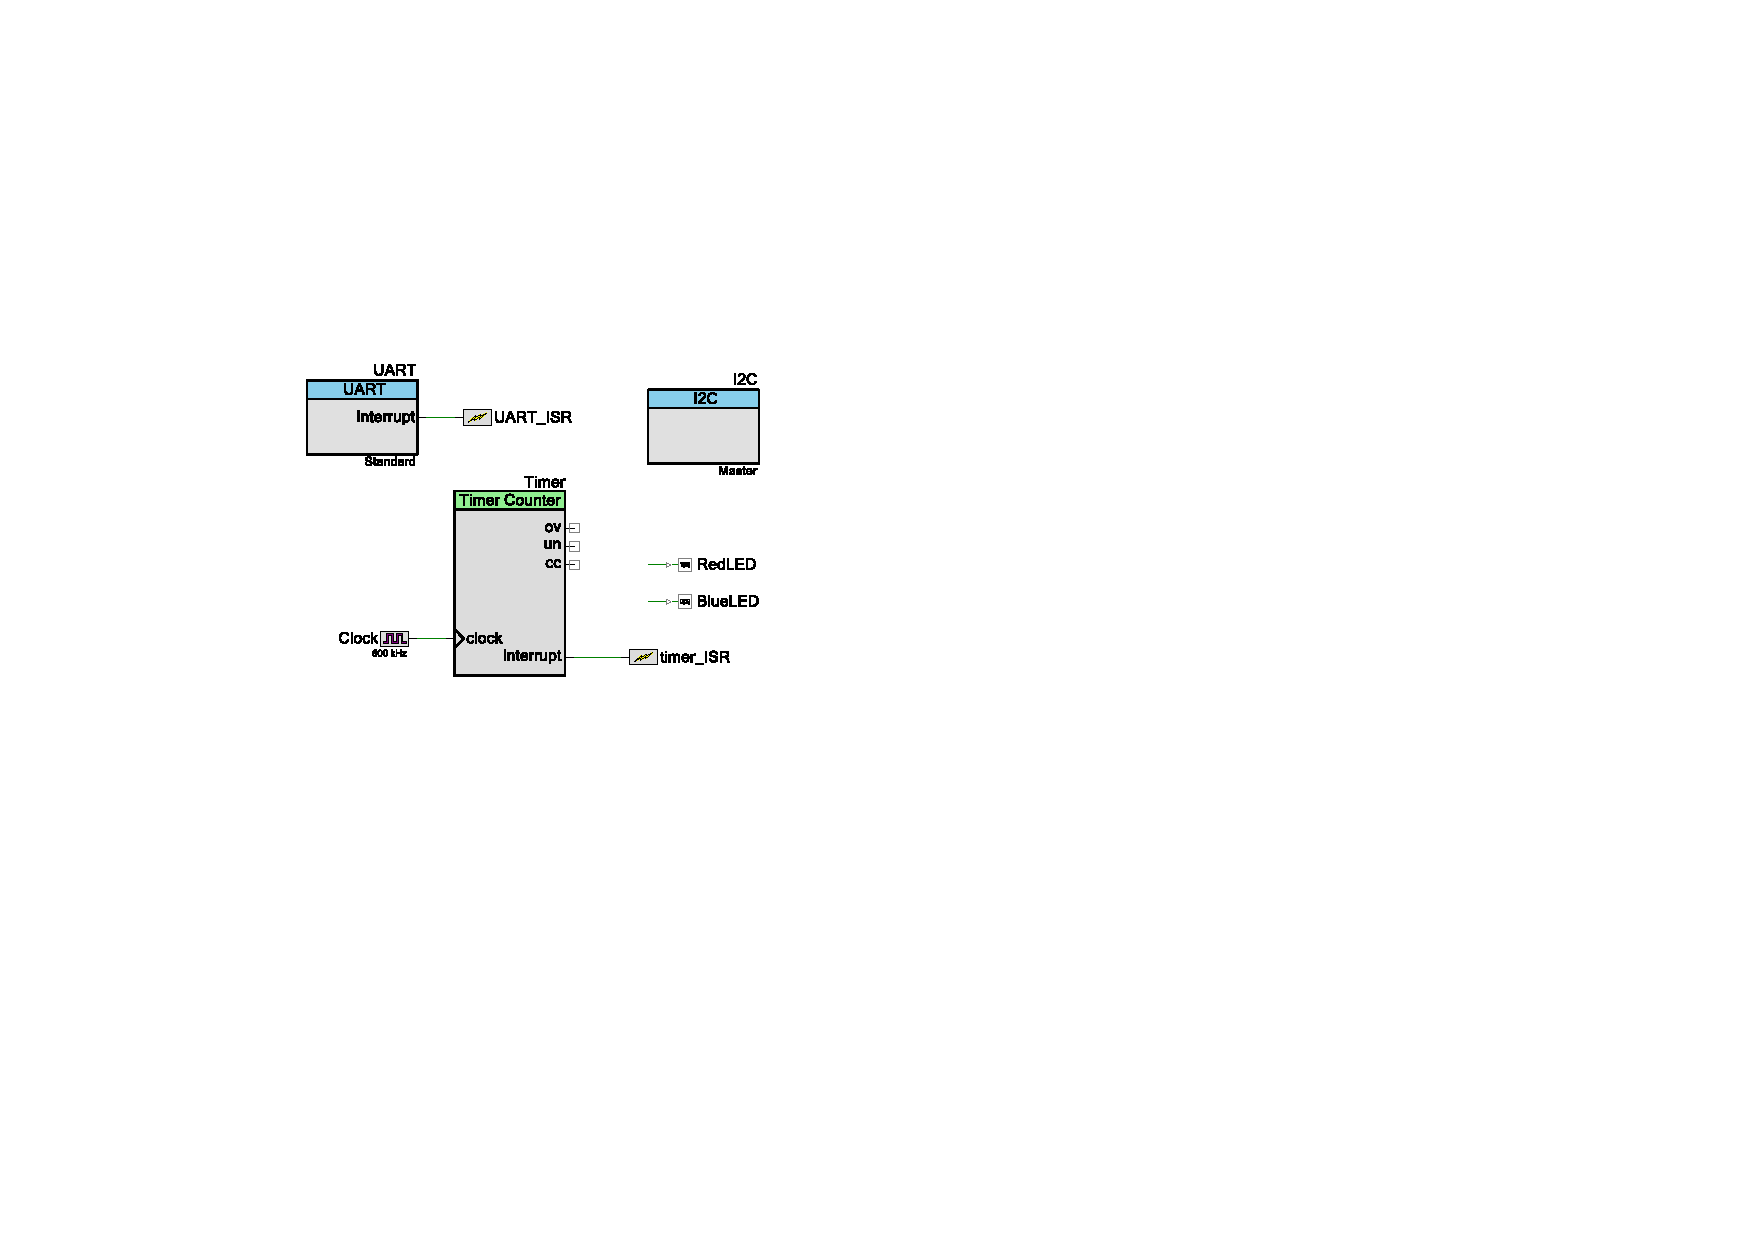
\includegraphics[width=\textwidth*3/5, trim=145 270 475 170, clip=true]{../fig/TopDesign_PSoC_Master}
\label{fig:psoc_master_topdesign}
\caption{TopDesign.cysch for PSoC\_Master}
\end{figure}

\subsection{\IIC implementering}

I forbindelse med implementeringen af \IIC klassen, blev prototyperne oprettet jf. \IIC protokollen (se side \pageref{sec:I2C_protokol}). Klassen reagerer på kald fra timer interruptet, og er i stand til at sende og indhente information hhv. til og fra sensorer og aktuatorer der er tilkoblet \IIC-bussen. Det blev valgt fra start af at den mest ideelle metode at få data mellem slaver og master, er altid at sørge for at der er noget data klar til at blive sendt. Pga. dette er der behov for at timer interrupten kan kalde \IIC-klassens metoder og derved opdatere de værdier der skal indhentes til DSP klassen. Desuden er der nødt til at blive taget højde for en forespørgsel om at åbne vinduet

\subsection{UART implementering}
UART klassen har til formål at modtage kommandoer fra DevKit8000, tolke disse og give passende svar. 

Generelt set er klassen implementering med udgangspunkt i vores UART protokol, men er udvidet således at der let kan implementeres flere trin i hhv. kontrol af vindue, motor og vanding. UART klassen gør brug af UART komponenten (SCB) vist i Figur \ref{fig:psoc_master_topdesign}.

\begin{lstlisting}[language=C,caption=Implementering af respondTemp(),label=lst:psoc_master_respondTemp]
int8 respondTemp(uint8 temp){
    if(temp){
        // If temp is between 1 and 200(both inclusive) "T" and temp is sent to DevKit8000
        UART_UartPutChar('T');
        UART_UartPutChar(temp);
        return 0;
    }
    else{
        // If temp isn't between 1 and 200(both inclusive) "XT" is sent to DevKit8000
        UART_UartPutChar('X');
        UART_UartPutChar('T');
        return -1;
    }
}
\end{lstlisting}

I Listing \ref{lst:psoc_master_respondTemp} vises et eksempel på en af funktionerne der håndterer svar via UART. De øvrige funktioner i klassen fungerer på samme måde. Funktionen modtager den værdi, der skal sendes tilbage til DevKit8000. Hvis parametren er 0 vil det sige at der er sket en fejl. Når funktionen kaldes kaldes den med returværdi fra DSP klassen, som beskrevet i afsnit \ref{sec:DSP_impl}.

\begin{lstlisting}[language=C, caption=Implementering af dkRequest(), label=lst:psoc_master_dkreq]
uint8 dkRequest(void){
    // Reads the UART buffer
    return UART_UartGetChar();
}
\end{lstlisting}

Vi har ydermere valgt at indkapsle læsningen fra UART ved hjælp af dkRequest() funktionen vist i Listing \ref{lst:psoc_master_dkreq}. Grunden til at vi har valgt at implementere denne er for at sikre os at hvis UART protokollen skulle ændre sig i fremtiden, kan disse ændringer tages højde for i denne funktion inden PSoC Master controllerklassen skal håndtere input fra UART.

\subsection{DSP implementering}\label{sec:DSP_impl}
DSP klassen agerer både digital signal processor og domæneklasse for vores måledata. Hver type af data er gemt i sit eget array, som vist i Listing \ref{lst:DSP_decl}. Hvert arrays har ligeledes en pointer til den næste plads i arrayet der skal overskrives.

\begin{lstlisting}[language=C, label=lst:DSP_decl, caption=Deklaration af arrays og pointers]
// Private data members
int32 tempArray[ARRAYSIZE];
int32* tempArrayPtr;
int32 humArray[ARRAYSIZE];
int32* humArrayPtr;
int16 soilHumArray[NBR_OF_SOILHUM_SENSORS][ARRAYSIZE];
int16* soilHumPtr[NBR_OF_SOILHUM_SENSORS];
int32 lightArray[ARRAYSIZE];
int32* lightArrayPtr;
uint8 temp, hum, soilHum[NBR_OF_SOILHUM_SENSORS], light;     // Used for storing the newest value
\end{lstlisting}



\subsection{Controller implementering}

